
% Copyright (c) 2015 - 2019 Mario Mlačak, mmlacak@gmail.com
% Licensed and published as Public Domain work.

% Conquest of Tlalocan chapter ========================================
\chapter*{Conquest of Tlalocan}
\addcontentsline{toc}{chapter}{Conquest of Tlalocan}

\begin{flushright}
\parbox{0.8\textwidth}{
\emph{The human mind is inspired enough when it comes to inventing
horrors; it is when it tries to invent a Heaven that it shows itself
cloddish. \\
\hspace*{\fill}{\textperiodcentered \textperiodcentered \textperiodcentered \hspace*{0.2em} Evelyn Waugh} } }
\end{flushright}

\noindent
Conquest of Tlalocan is chess variant which is played on 24 x 24 board,
with bright red and cyan fields, and dark red and light green pieces.
Star colors are bright red and bright blue. In algebraic notation, columns
are enumerated from 'a' to 'x', and rows are enumerated from '1' to '24'.
A new piece is introduced, Shaman.

\clearpage % ..........................................................
% Shaman **************************************************************

\section*{Shaman}
\addcontentsline{toc}{section}{Shaman}

\noindent
\begin{wrapfigure}[11]{l}{0.4\textwidth}
\centering
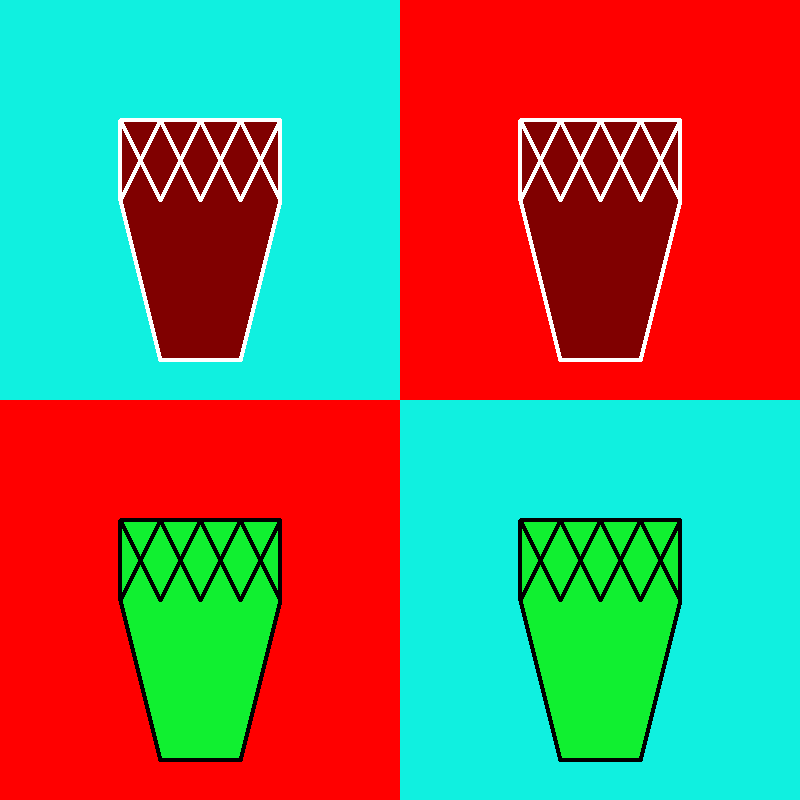
\includegraphics[width=0.4\textwidth, keepaspectratio=true]{pieces/14_shaman.png}
\caption{Shaman}
\label{fig:14_shaman}
\end{wrapfigure}
Shaman moves like sort-of cross between Knight and long-jump Unicorn,
where one figure provides step-fields, and the other capture-fields.

For light Shaman, step-fields are provided by the Knight, while capture-fields
are provided by long-range Unicorn. For dark Shaman, it's the opposite.

Shaman can continue it's jumpy movement in chosen direction; over step-fields
if they're empty, over capture-fields as long as it's capturing opponent's
pieces. Shaman can't change direction once started moving.

Shaman can activate both Wave and Pyramid on its' capture-fields, while only
Wave can be activated on step-fields.

% \vspace*{0.05\textheight}
\noindent
\begin{wrapfigure}{l}{0.4\textwidth}
\centering
\includegraphics[width=0.4\textwidth, keepaspectratio=true]{pieces/star/18_conquest_of_tlalocan.png}
\caption{Star}
\label{fig:star/18_conquest_of_tlalocan}
\end{wrapfigure}
Alternative move for Shaman is a trance-journey.

Shaman symbol in algebraic notation is 'H', to avoid confusion with Serpent.

Star colors in this variant are presented on the left.

\clearpage % ..........................................................
% Movement ------------------------------------------------------------

\subsection*{Movement}
\addcontentsline{toc}{subsection}{Movement}

\noindent
\begin{figure}[!h]
% \begin{figure}[!t]
\includegraphics[width=1.0\textwidth, keepaspectratio=true]{examples/18_cot/scn_cot_01_shaman_movement.png}
\caption{Shaman's movement}
\label{fig:scn_cot_01_shaman_movement}
% \centering
\end{figure}

For this variant examples are rendered in B\&W to improve legibility.
Here, step-fields are marked green, while capture-fields are marked blue.
Note, movement of Shaman does not depend on color of field on which it
stands, only on color of the piece itself.

\clearpage % ..........................................................

\noindent
\begin{figure}[!h]
% \begin{figure}[!t]
\includegraphics[width=1.0\textwidth, keepaspectratio=true]{examples/18_cot/scn_cot_02_light_shaman_step_ply.png}
\caption{Light Shaman's step-ply}
\label{fig:scn_cot_02_light_shaman_step_ply}
% \centering
\end{figure}

Once initial step-direction is chosen, light Shaman has to follow it,
and so moves similar to Pegasus. Unlike Pegasus, Shaman can't capture
opponent's pieces on step-fields, nor activate Pyramid. Wave on step-field
can be activated, and would continue to move as Shaman (and Pegasus)
would. Again, once direction is chosen, it cannot be changed, neither
in other step- nor capture-direction, even if opponent's piece is present
on capture-field.

\clearpage % ..........................................................

\noindent
\begin{figure}[!h]
% \begin{figure}[!t]
\includegraphics[width=1.0\textwidth, keepaspectratio=true]{examples/18_cot/scn_cot_03_light_shaman_capture_ply.png}
\caption{Light Shaman's capture-ply}
\label{fig:scn_cot_03_light_shaman_capture_ply}
% \centering
\end{figure}

Capture-ply can only be started with immediate capture, after which Shaman
can continue its' movement as long as it's keep capturing opponent's pieces
in the same direction. Empty capture-fields cannot be oversteped, any piece
at a distance is out of reach. Again, once started capturing, Shaman cannot
change it's heading, neither in other step- nor capture-direction. Shaman
can also activate Pyramid or Wave on capture-field, thus ending it's ply.

\clearpage % ..........................................................

\noindent
\begin{figure}[!h]
% \begin{figure}[!t]
\includegraphics[width=1.0\textwidth, keepaspectratio=true]{examples/18_cot/scn_cot_04_dark_shaman_step_ply.png}
\caption{Dark Shaman's step-ply}
\label{fig:scn_cot_04_dark_shaman_step_ply}
% \centering
\end{figure}

Dark Shaman's step-ply is the same as light Shaman's, except it steps like a
long-jump Unicorn, in chosen direction. Shaman can't capture opponent's pieces
on step-fields, nor activate Pyramid. Wave on step-field can be activated, and
would continue to move as dark Shaman would. Again, once direction is chosen,
it cannot be changed, neither in other step- nor capture-direction, even if
opponent's piece is present on capture-field.

\clearpage % ..........................................................

\noindent
\begin{figure}[!h]
% \begin{figure}[!t]
\includegraphics[width=1.0\textwidth, keepaspectratio=true]{examples/18_cot/scn_cot_05_dark_shaman_capture_ply.png}
\caption{Dark Shaman's capture-ply}
\label{fig:scn_cot_05_dark_shaman_capture_ply}
% \centering
\end{figure}

Dark Shaman's capture-ply is the same as light Shaman's, except it captures like
Pegasus, in chosen direction. Capture-ply can be initiated with immediate capture,
after which Shaman can continue capturing opponent's pieces, in the same direction,
if there is no empty capture-field in-between. While capturing, Shaman cannot change
it's heading to any other direction. Shaman can also activate Pyramid or Wave on
capture-field, thus ending it's ply.

\clearpage % ..........................................................

\subsubsection*{Activating Wave}
\addcontentsline{toc}{subsubsection}{Activating Wave}

\noindent
\begin{figure}[!h]
% \begin{figure}[!t]
\includegraphics[width=1.0\textwidth, keepaspectratio=true]{examples/18_cot/scn_cot_06_wave_activated.png}
\caption{Shaman activated Wave}
\label{fig:scn_cot_06_wave_activated}
% \centering
\end{figure}

If activated on Shaman's capture-field, similar to being activated on
step-field, Wave can choose freely any Shaman's initial capture-field
as a heading, and then continue it's movement in chosen direction,
possibly ending it by activating other piece.

% ------------------------------------------------------------ Movement
\clearpage % ..........................................................
% Trance-journey ------------------------------------------------------

\subsection*{Trance-journey}
\addcontentsline{toc}{subsection}{Trance-journey}

\noindent
\begin{wrapfigure}[1]{l}{0.35\textwidth} % [11]
\centering
\includegraphics[width=0.3333333333333333\textwidth, keepaspectratio=true]{examples/18_cot/scn_cot_07_trance_init.png}
\caption{Start}
\label{fig:scn_cot_07_trance_init}
\end{wrapfigure}
...

\vspace*{0.25\textheight}
\subsubsection*{Movement}
\addcontentsline{toc}{subsubsection}{Movement}

\noindent
\begin{wrapfigure}{l}{0.4\textwidth} % [11]
\centering
\includegraphics[width=0.375\textwidth, keepaspectratio=true]{examples/18_cot/scn_cot_08_knight_directions.png}
\caption{Knight directions}
\label{fig:scn_cot_08_knight_directions}
\end{wrapfigure}
...

\clearpage % ..........................................................

\noindent
\begin{wrapfigure}{l}{0.4\textwidth} % [11]
\centering
\includegraphics[width=0.375\textwidth, keepaspectratio=true]{examples/18_cot/scn_cot_09_stop_sign_pattern.png}
\caption{Stop sign pattern}
\label{fig:scn_cot_09_stop_sign_pattern}
\end{wrapfigure}
...

\vspace*{0.35\textheight}
\noindent
\begin{wrapfigure}{l}{0.4\textwidth} % [11]
\centering
\includegraphics[width=0.375\textwidth, keepaspectratio=true]{examples/18_cot/scn_cot_10_stop_sign_pattern_unwind.png}
\caption{Stop sign pattern unwinded}
\label{fig:scn_cot_10_stop_sign_pattern_unwind}
\end{wrapfigure}
...

\clearpage % ..........................................................

\noindent
\begin{figure}[!h]
% \begin{figure}[!t]
\includegraphics[width=1.0\textwidth, keepaspectratio=true]{examples/18_cot/scn_cot_12_light_shaman_trance_journey.png}
\caption{Light Shaman trance-journey}
\label{fig:scn_cot_12_light_shaman_trance_journey}
% \centering
\end{figure}

...

\clearpage % ..........................................................

\noindent
\begin{figure}[!h]
% \begin{figure}[!t]
\includegraphics[width=1.0\textwidth, keepaspectratio=true]{examples/18_cot/scn_cot_13_dark_shaman_trance_journey.png}
\caption{Dark Shaman trance-journey}
\label{fig:scn_cot_13_dark_shaman_trance_journey}
% \centering
\end{figure}

...

\clearpage % ..........................................................

\subsubsection*{Interaction}
\addcontentsline{toc}{subsubsection}{Interaction}

...

\clearpage % ..........................................................

\subsubsection*{Push-pull entrancement}
\addcontentsline{toc}{subsubsection}{Push-pull entrancement}

...




% ------------------------------------------------------ Trance-journey
% ************************************************************** Shaman
\clearpage % ..........................................................

\section*{Promotion}
\addcontentsline{toc}{section}{Promotion}

Promotion is non enforced, delayed variety, i.e. it's the same as in
\hyperref[sec:Age of Aquarius/Promotion]{previous chess variant}, Age of Aquarius.

Promotion in this variant is polygamous, more than one Queen in the same color
can be present on chessboard at any given time.

\clearpage % ..........................................................

\section*{En passant}
\addcontentsline{toc}{section}{En passant}

\noindent
\begin{wrapfigure}{l}{0.4\textwidth}
\centering
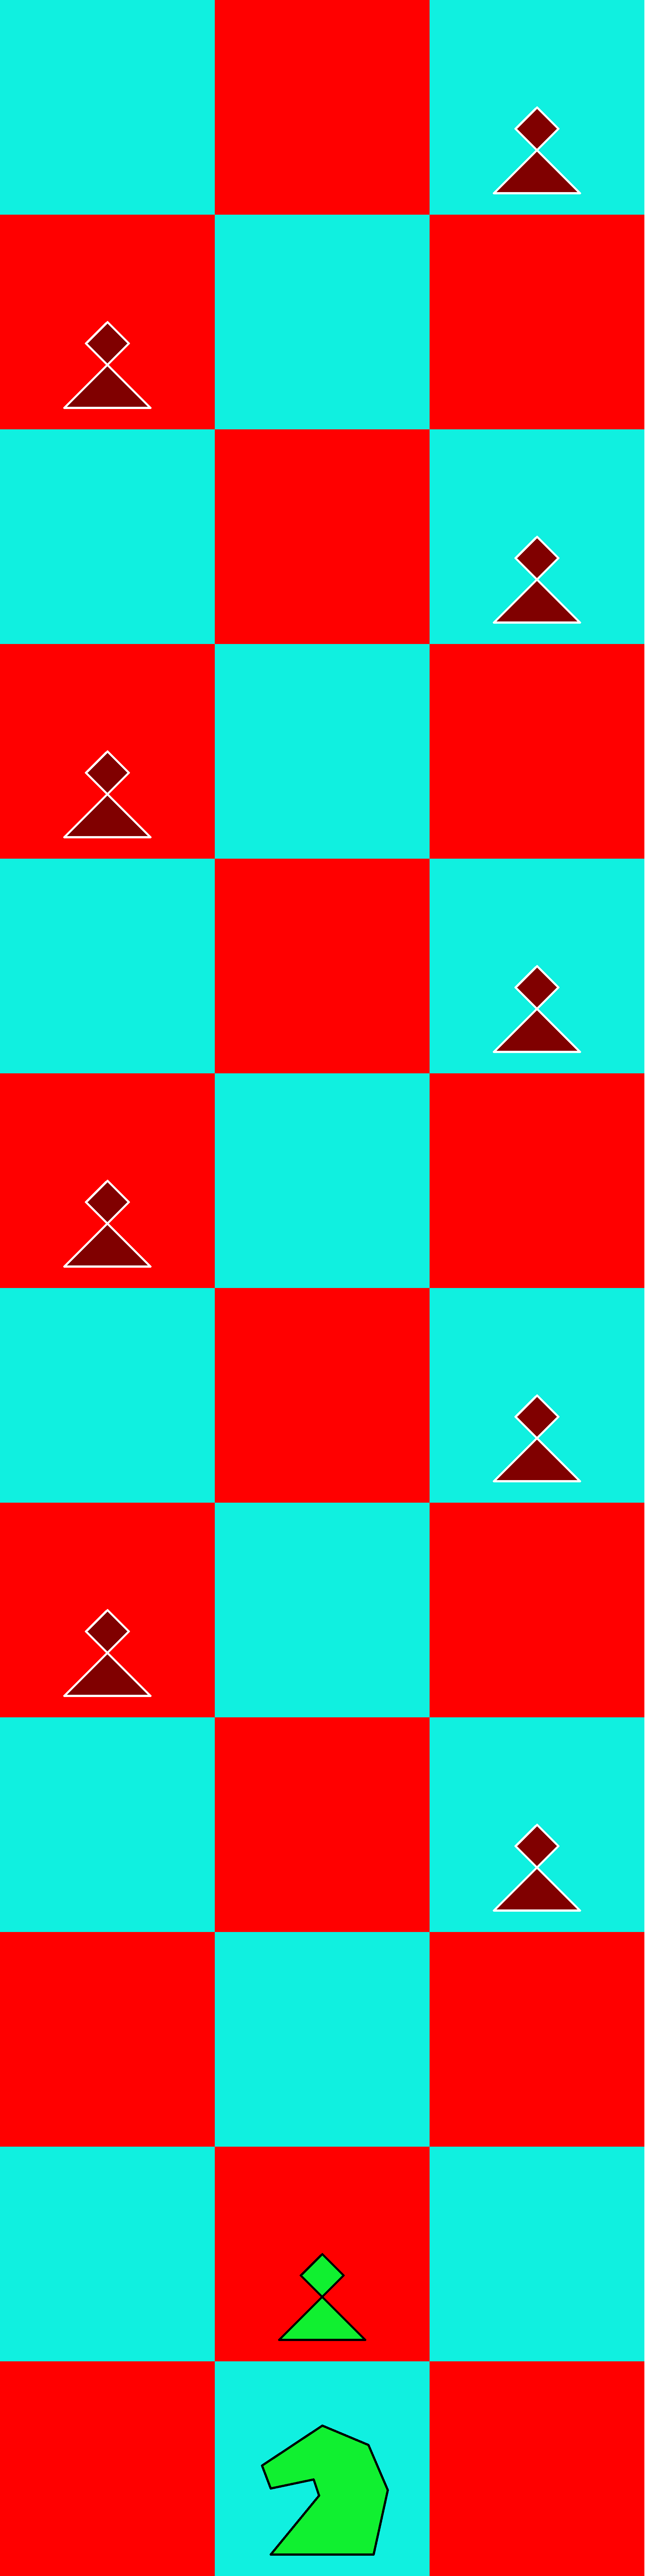
\includegraphics[width=0.125\textwidth, keepaspectratio=true]{en_passants/18_conquest_of_tlalocan_en_passant.png}
\caption{En passant}
\label{fig:18_conquest_of_tlalocan_en_passant}
\end{wrapfigure}
Rush and en passant are identical to those in Classic Chess, only difference
is that Pawn can now move longer on initial turn, up to 9 fields in this
variant.

\clearpage % ..........................................................

\section*{Castling}
\addcontentsline{toc}{section}{Castling}

Castling is the same as in Classical Chess, only difference is that King can move between 2 and 8 fields across.
All other constraints from Classical Chess still applies.

\noindent
\begin{figure}[!h]
% \begin{figure}[!t]
\includegraphics[width=1.0\textwidth, keepaspectratio=true]{castlings/18_cot/conquest_of_tlalocan_castling.png}
\caption{Castling}
\label{fig:conquest_of_tlalocan_castling}
% \centering
\end{figure}

In example above, all valid King's castling moves are numbered.

\noindent
\begin{figure}[!h]
% \begin{figure}[!t]
\includegraphics[width=1.0\textwidth, keepaspectratio=true]{castlings/18_cot/conquest_of_tlalocan_castling_right_08.png}
\caption{Castling long right}
\label{fig:conquest_of_tlalocan_castling_right_08}
% \centering
\end{figure}

In this example King was castling long to the right. Initial King's position is marked with "K".
After castling is finished, right Rook ends up at field immediately left to the King.

\clearpage % ..........................................................

\section*{Initial setup}
\addcontentsline{toc}{section}{Initial setup}

Compared to initial setup of Tamoanchan Revisited, Shaman is inserted between Unicorn and Pyramid
symmetrically, on both sides of chessboard. This can be seen in the image below:

\noindent
% \begin{figure}[t]
\begin{figure}[h]
\includegraphics[width=1.0\textwidth, keepaspectratio=true]{boards/18_conquest_of_tlalocan.png}
\caption{Conquest of Tlalocan board}
\label{fig:18_conquest_of_tlalocan}
% \centering
\end{figure}

\clearpage % ..........................................................
% ======================================== Conquest of Tlalocan chapter
